\subsection{Effect of Memory Bandwidth Throttling}

To determine the how sensitive the model is to the shared DRAM 
memory, we use MemGuard\cite{yun2014rtas}, a memory bandwidth reservation system that 
can limit the amount of bandwidth each core receives in a period. For 
all tests run using MemGuard, we use a period of one second. 

\begin{figure}[h]
  \centering
  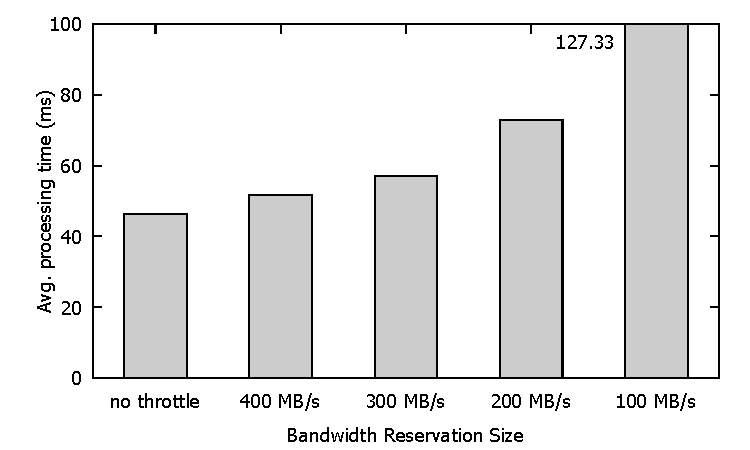
\includegraphics[width=.45\textwidth]{figs/memguard_multicore}
  \caption{ Memory bandwidth sensitivity of the control loop 
execution time. }
  \label{fig:memguard_multicore}
\end{figure}

We first run a single model on one core, Core 0, while varying the 
core's bandwidth reservation size, from 500 MB/s down to 100 MB/s. 
The results can be seen in Figure \ref{fig:memguard_multicore}. When less 
memory bandwidth is available to the core the model's performance 
noticably decreases.
%% , and it performs the best when no memory bandwidth 
%% throttling is implemented. 
Compared to a reservation size of 100 
MB/s, disabling memory bandwidth throttling results in 
\textasciitilde3x performance improvement. If the model was memory 
insensitive, then the amount of bandwidth available to it would have 
little effect on its performance. However, since that is not the 
case, we conclude that, to a notable extent, the neural network model 
is dependent on shared DRAM memory performance.

%% \begin{figure}[h]
%%   \centering
%%   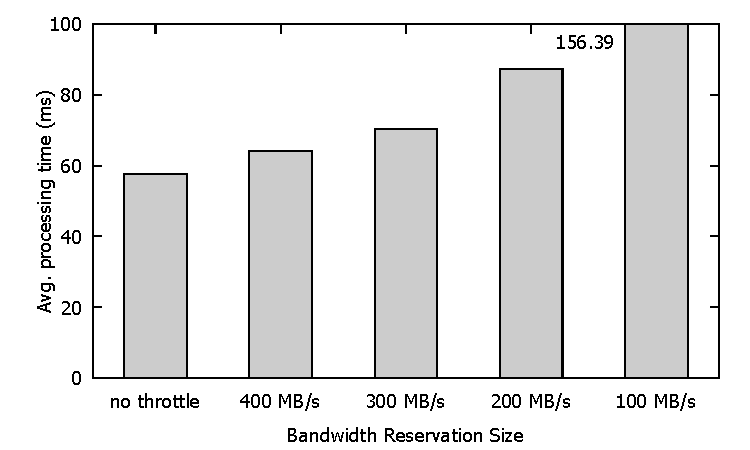
\includegraphics[width=.45\textwidth]{figs/memguard_multimodel}
%%   \caption{Timing impact of co-scheduling multiple DNNs when memory
%% bandwidth throttling is enabled. }
%%   \label{fig:memguard_multimodel}
%% \end{figure}

%% We also test the effects of memory bandwidth throttling in the case 
%% of multiple models running concurrently on the Pi 3 by rerunning the 
%% 4Nx1C experiment. We use the same memory bandwidth reservation sizes 
%% from the previous experiment. The results can be seen in Figure
%% \ref{fig:memguard_multimodel}. Once again, the performance of the 
%% models are affected by the amount of memory bandwidth that is 
%% available to the Pi 3's cores during each period, meaning that they 
%% are all memory dependent.

\begin{figure}[h]
  \centering
  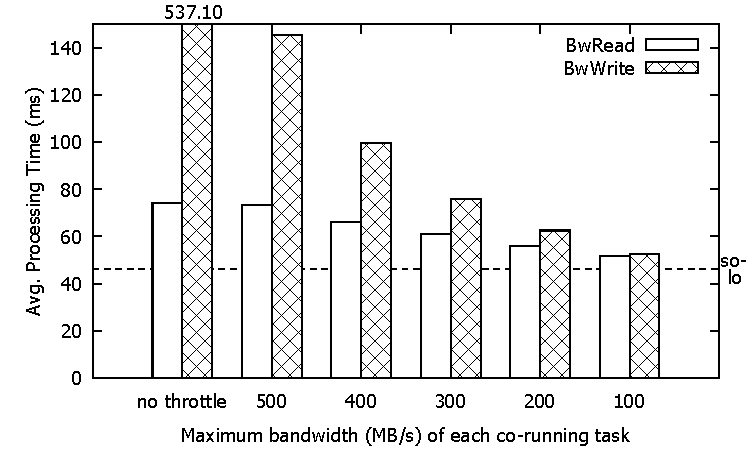
\includegraphics[width=.45\textwidth]{figs/memguard_bandwidth}
  \caption{Timing impact of co-scheduling memory intensive read
co-runners when memory bandwidth throttling is enabled. }
  \label{fig:memguard_bandwidth}
\end{figure}

\begin{figure}[h]
  \centering
  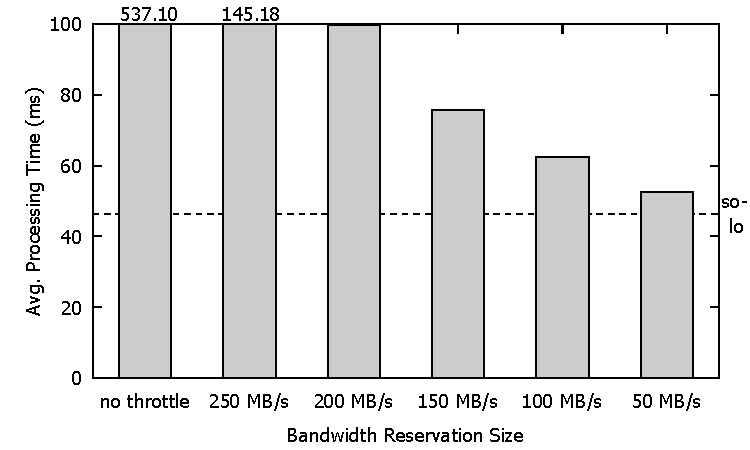
\includegraphics[width=.45\textwidth]{figs/memguard_bwwrite}
  \caption{Timing impact of co-scheduling memory intensive write
co-runners when memory bandwidth throttling is enabled. }
  \label{fig:memguard_bwwrite}
\end{figure}

We also test the performance of the model in the presence of three
memory intensive read and write benchmarks to determine the effects of 
limiting the memory bandwidth of the co-runners. For each of the 
experiments, we give the model's core, Core 0, a constant 1000 MB/s 
memory bandwidth reservation size, and then vary the amount of bandwidth 
the co-runners' cores receive. For read co-runners, we give them an initial
reservation size of 500 MB/s, and decrease that to a minimum of 100 MB/s.
In the case of write co-runners, MemGuard accounts for L2 refills but not
write-backs, so each benchmark would effectively have twice the bandwidth
of their reservation size. Due to this, we give write co-runners an initial 
reservation size of 250 MB/s and decrease it to a minimum of 50 MB/s.
The results can be see in Figures \ref{fig:memguard_bandwidth} and
\ref{fig:memguard_bwwrite}. When less memory bandwidth is given to 
the both the  read and write co-runners, the performance of the model 
improves. 
%% In the case of one co-runner, the performance of the model remains 
%% constant even as the reservation sizes are decreased, however, it 
%% still improves compared to when throttling wasn't enabled. 
In both cases, when the co-runners were given a minimal reservation size,
the performance of the model was much closer to its solo execution time.
This is especially noteworthy when write co-runners were present, as the 
model didn't suffer the same 11.6X slowdown that was seen without
bandwidth throttling enabled. 
%% When memory intensive Bandwidth benchmarks were present, model performance
%% improved, to a notable extent, through the use of memory bandwidth 
%% throttling on the co-runners. 
Since this would not be the case if the 
model was memory insensitive, we find that the model is memory 
dependent in the presence of co-runners.

Based on all of the memory bandwidth throttling experiments 
performed, it is evident that the shared DRAM memory is important for
the DNN model. When a single model was run, its 
performance decreased as less memory bandwidth was 
made available to it. Furthermore, when the bandwidths of memory 
intensive read and write co-runners were limited, the performance of 
the model improved. As such, we conclude that the model is dependent on the 
shared DRAM memory.